\documentclass[11pt,a4paper]{article}

\usepackage[utf8]{inputenc}
\usepackage[T1]{fontenc}
\usepackage{amsmath,amssymb}
\usepackage{booktabs}
\usepackage{graphicx}
\usepackage{longtable}
\usepackage{url}
\usepackage[margin=1in]{geometry}
\usepackage[hidelinks]{hyperref}

\newcommand{\code}[1]{\texttt{\small #1}}

\title{Measured Self-Occlusion in a Deployed Cross-Sensor Diagnostic Layer:\\
When a Fault Destroys the Evidence That Would Name It}

\author{SWORT Aerospace}
\date{}

\begin{document}
\maketitle

\begin{abstract}
We report a measurement on a deployed cross-sensor diagnostic layer for small
uncrewed aircraft. The layer maintains per-sensor trust coefficients over a
physics-derived graph and runs a gated naive-Bayes diagnosis over eight
mutually exclusive causes. Each diagnostic feature carries a validity gate,
and a gated feature is skipped rather than down-weighted. One gate,
GPS fix validity, is closed by the very fault it helps diagnose. We measure
the consequence on the running system: under sustained GPS denial the
diagnosis reports \code{nominal} for the entire 40\,s fault window, never once
naming \code{gps\_fault}, while the GPS trust coefficient reads 0.9767, above
the actionable threshold. The vehicle is not blind to the condition. Its
failsafe reaches CAUTION through an independent data-freshness disjunct and
issues navigation-reconfiguration actions. It cannot, however, name the cause.
We report the structural condition under which this is irreparable by adding
evidence, a chatter-resonance prediction tested against the deployed code and
holding, a one-line repair to a second collision with its full measured cost,
and a design-rule check now enforced in the project's test suite. We claim
engineering contribution and measurement only. The frameworks that describe
diagnosis under mode-dependent or unreliable observation already exist and are
cited as the ones this work instantiates.
\end{abstract}

%======================================================================
\section{Introduction}
\label{sec:intro}

Model-based diagnosis on a real vehicle rarely evaluates every residual at
every instant. Residuals are gated: a cross-check between barometric and GNSS
altitude is meaningless without a GNSS fix, and a thrust-versus-current
relation is meaningless before the motors are armed. Gating is correct
engineering. It is also where a specific failure mode lives.

The failure mode is this. If a fault closes a gate, and the features that gate
controls are the only evidence for that fault, then the fault removes its own
evidence. Nothing in the diagnosis reports an anomaly, because the anomalous
feature is not evaluated at all. The system does not become uncertain. It
becomes confident, and wrong, in the direction of health.

We measured it. On the deployed layer, with a GPS denial fault active for
40\,s, the diagnosis reported \code{nominal} on 100\% of post-onset ticks and
reached \code{gps\_fault} zero times. The GPS trust coefficient over the same
window never fell below 0.9767, because a channel that stops delivering data
has its belief update frozen rather than driven down: absence of evidence is
not treated as evidence of fault. Both the attribution channel and the trust
channel independently reported health while a fault the layer was built to
catch was active.

\textbf{The vehicle is not blind to the condition, and we state that before
any reader can form a wrong impression.} The failsafe policy escalates to
CAUTION and issues \code{SWITCH\_NAV\_INERTIAL} and \code{INHIBIT\_GPS\_MODES}
in this scenario, driven by a data-freshness disjunct that does not consult the
diagnosis. The gap is in attribution, not in escalation. What is lost is the
ability to name the cause, and therefore the ability to choose a
cause-specific response, to log a correct incident record, or to distinguish
GNSS denial from a benign loss of reception.

\textbf{The condition is narrower than the failure mode described above, and
we bound it here rather than in the limitations.} A controlled-injection
campaign against a full ArduPilot autopilot
(Section~\ref{sec:qgvalid}) finds that faults which remove the GNSS fix close
the gate almost always, and that a 62 to 76\,m position glitch which keeps the
fix does not close it at all. Self-occlusion is a property of fix-loss faults,
not of GNSS faults in general.

We make no mathematical claim. Diagnosis under intermittent and permanent loss
of observations is established
\cite{carvalho2012intermittent,carvalho2013permanent}, as is diagnosability
under state-dependent observation \cite{yin_phidiagnosability} and, for the
fault-state-dependent case that ours is an instance of,
\cite{dong2024statedependent}. Structural isolability with mode-dependent
signatures is established
\cite{krysander2024multimode,krysander2008sensorplacement}, and the
reliability-side machinery we apply is likewise established
\cite{hurdle2007faulttree,reeves2019sensorselection}. Our contribution is a
measurement on a real system, an engineering rule derived from it, and a
repair whose cost we report.

%======================================================================
\section{Related work: what we instantiate}
\label{sec:related}

We list, for each framework, what we take from it and what we do not claim.

\paragraph{Diagnosis under unreliable observation.}
Carvalho et al. treat diagnosability when observations are lost intermittently
\cite{carvalho2012intermittent} and permanently
\cite{carvalho2013permanent}, including the case where the diagnoser is
unaware that a sensor has failed. \emph{What we take}: the framing that
observation availability is part of the diagnosis problem rather than a
precondition of it. \emph{What we claim}: nothing. Our gate closure is an
instance of observation loss in their sense.

\paragraph{State-dependent observation maps.}
Yin et al.\ develop diagnosability when the observation map depends on system
state \cite{yin_phidiagnosability}. \emph{What we take}: the recognition that
a hypothesis-dependent observation map is a studied object.
\emph{What we claim}: nothing.

\paragraph{Fault-state-dependent observation loss.}
Dong, Yin and Li verify diagnosability under a state-dependent observation map
$O: Q \times \Sigma \to 2^{\Delta \cup \{\varepsilon\}}$, which permits the
observation available at a transition to depend on the state the system is in,
including a fault state \cite{dong2024statedependent}. Our situation maps onto
theirs directly: a fault-labelled augmented state corresponds to the hypothesis
being active, $O(q,\sigma) = \{\varepsilon\}$ corresponds to gate closure
silencing a feature, and failure of $\varphi$-diagnosability corresponds to
what we call effective undetectability. \emph{What we take}: the general
mechanism of fault-induced observation suppression, entire.
\emph{What we claim}: nothing. Priority for general fault-induced suppression
belongs to them. What is left to us is a measurement on a deployed system and
a scoped enumeration of one system's evidence set, neither of which is a
statement about the general mechanism.

\paragraph{Structural isolability and mode-dependent signatures.}
Krysander and colleagues compute isolability from structural models and select
residuals that preserve diagnosability across operating modes
\cite{krysander2024multimode}, and compute minimal sensor sets for an
isolability specification \cite{krysander2008sensorplacement}. \emph{What we
take}: the design-time signature matrix and its induced partition, which we
use as the baseline our measurement is compared against. \emph{What we claim}:
nothing. Our design-time analysis is theirs.

\paragraph{Fault trees and sensor selection by diagnostic performance.}
Hurdle et al.\ apply fault-tree methods to diagnosing system operation
\cite{hurdle2007faulttree}; Reeves et al.\ select sensors against a diagnostic
performance metric \cite{reeves2019sensorselection}. \emph{What we take}: the
whole apparatus of Section~\ref{sec:repair}'s cut-set analysis, unchanged.
\emph{What we claim}: nothing. Applying coherent-system structure functions to
diagnostic capability is their contribution, not ours.

\paragraph{Isolation to the granularity of reconfiguration.}
Blanke et al.\ establish that faults need only be distinguished to the
granularity that the reconfiguration map requires \cite{blanke2003ftc}. We use
this to define the decision-relevant pair set in
Section~\ref{sec:system}. \emph{What we claim}: nothing.

%======================================================================
\section{System under measurement}
\label{sec:system}

The layer maintains a trust coefficient $T_i \in (0,1)$ per sensor node over a
graph of 8 nodes and 11 physics-derived edges. Each edge and each per-node
physics self-model produces a chi-square-normalised residual $\lambda$, mapped
to a consistency score
\begin{equation}
c = \exp\!\left(-\tfrac{1}{2}\max(0, \lambda - 1)\right),
\end{equation}
so that only excess over the chi-square nominal penalises trust. Fused
evidence updates a Beta belief with adaptive forgetting $\rho \in [0.95,
0.998]$, and the belief update is skipped entirely when a channel's data is
stale.

Diagnosis is a gated naive Bayes over 8 mutually exclusive hypotheses. Each
feature $f$ carries a gate $g_f \in [0,1]$, and the accumulation is
\begin{equation}
\ell_h \mathrel{+}= g_f \cdot
\begin{cases}
\log(1 - c_f + \varepsilon) & f \in \mathrm{LOW}(h)\\
\log(c_f + \varepsilon) & \text{otherwise,}
\end{cases}
\qquad \varepsilon = 0.02,
\end{equation}
followed by exponential smoothing with $\alpha_s = 0.06$, tempering by 1.5,
and a softmax against a prior placing 0.86 on \code{nominal}.

\textbf{The load-bearing implementation detail} is that a feature with
$g_f \le 10^{-9}$ is skipped by a \code{continue}, not down-weighted. It
therefore contributes to no hypothesis. Two hypotheses whose LOW sets coincide
over the surviving features accumulate identical likelihood indefinitely, and
their posterior ratio remains pinned at the prior ratio. This is
indistinguishability, not weak evidence.

\subsection{Gates}

Fourteen gates exist. Eight are data-freshness gates that block a node's
belief update rather than any named feature. Two are compile-time constants
that never actuate. Four vary with vehicle state and control a feature that
some hypothesis references:

\begin{table}[h]
\centering
\small
\begin{tabular}{llll}
\toprule
Gate & Predicate & Controls & Closed by \\
\midrule
\code{armed\_gate} & arming state, 1\,s ramp & 2 motor edges & nothing \\
\code{gvalid} & GNSS fix valid & 5 features incl.\ \code{phys\_gps} &
  \code{gps\_fault} \\
\code{speed\_gate} & ground speed 2--3\,m/s & \code{heading\_course} &
  undetermined \\
\code{gps\_warmup} & elapsed time $>3$\,s & \code{phys\_gps} & nothing \\
\bottomrule
\end{tabular}
\caption{The four actuating gates. Closure attribution is derived from source
and the fault model; 29 of 32 hypothesis-gate cells are so derived, the three
undetermined cells all concern \code{speed\_gate} and none of them changes any
partition reported here.}
\end{table}

\subsection{Design-time and effective signatures}

Let $S[f,h]=1$ when hypothesis $h$ perturbs feature $f$. Write
$\mathrm{closes}(h,g)$ when $h$ drives gate $g$ closed, and define
\begin{equation}
S_{\mathrm{eff}}[f,h] = S[f,h] \wedge
\neg\big(\exists\, g \in \mathrm{gate}(f) : \mathrm{closes}(h,g)\big).
\label{eq:seff}
\end{equation}
A feature counts as evidence for $h$ only if $h$ perturbs it and does not
silence it. Since $S_{\mathrm{eff}} \le S$ entrywise, the induced partition
$\Pi(S_{\mathrm{eff}})$ is no finer than $\Pi(S)$. This is monotonicity of
distinguishability under deletion of observations and we do not present it as
more than that.

Applied to this system, with $\kappa = (H-P)/(H-1)$ for $H=8$ hypotheses and
$P$ observable classes:
$\kappa(S) = 0.000$ over 8 classes, and
$\kappa(S_{\mathrm{eff}}) = 0.143$ over 7 classes, the merged pair being
\code{gps\_fault} and \code{nominal}. The design-time artifact reports full
isolability for a system that does not have it.

\begin{table}[h]
\centering
\small
\begin{tabular}{llll}
\toprule
Hypothesis & LOW feature & Gated by & Closed by this hypothesis? \\
\midrule
\code{nominal} & (empty by definition) & --- & --- \\
\textbf{\code{gps\_fault}} & \textbf{\code{phys\_gps}} &
  \textbf{\code{gvalid}, \code{gps\_warmup}} & \textbf{yes, \code{gvalid}} \\
\code{imu0\_bias\_drift} & \code{redundant\_imu} & --- & no \\
 & \code{accel\_motor\_current} & \code{armed\_gate} & no \\
 & \code{attitude\_gravity\_mag} & --- & no \\
\code{imu1\_bias\_drift} & \code{redundant\_imu}, \code{accel\_esc\_rpm} &
  \code{armed\_gate} (2nd) & no \\
\code{mag\_interference} & 4 features & \code{gvalid}, \code{speed\_gate}
  (1 of 4) & no \\
\code{power\_fault} & 5 features & \code{armed\_gate} (2 of 5) & no \\
\code{vibration\_anomaly} & 3 features & --- & no \\
\code{unexpected\_maneuver} & \code{temp\_gps} & --- (ungated) & no \\
\bottomrule
\end{tabular}
\caption{$S$ and $S_{\mathrm{eff}}$ in one table. \code{gps\_fault} has one
feature, that feature is gated by \code{gvalid}, and a GPS fault closes
\code{gvalid}. Its $S_{\mathrm{eff}}$ column is empty, which is
\code{nominal}'s column.}
\label{tab:signatures}
\end{table}

\subsection{Decision-relevant pairs}

Following \cite{blanke2003ftc}, only distinctions that change the commanded
response matter. Reading the failsafe automaton's action table including action
parameters, 27 of the 28 hypothesis pairs are decision-relevant. The single
exception is \code{nominal} versus \code{unexpected\_maneuver}: both command
the empty action set. Note that \code{imu0\_bias\_drift} and
\code{imu1\_bias\_drift} raise the same condition but parameterise
\code{SELECT\_IMU} differently, so that pair is decision-relevant.

%======================================================================
\section{The self-occlusion measurement}
\label{sec:measurement}

Three arms, identical flight profile and seed, differing only in whether the
GPS fault destroys the fix. The failsafe is the shipping policy, driven from
the batch trust history by the adapter the project already ships for its
dashboard, so no policy logic is reimplemented.

\begin{table}[h]
\centering
\small
\begin{tabular}{lrrr}
\toprule
& A: spoof, fix valid & B: denial, fix invalid & C: spoof then denial \\
\midrule
\code{gvalid} closed, post-onset & 0\% & \textbf{62\%} & 50\% \\
\code{gps\_fault} on top & 66.5\% & \textbf{0.0\%} & 15.6\% \\
\code{nominal} on top & 33.5\% & \textbf{100\%} & 84.4\% \\
Time to first correct lead & 1.44\,s & \textbf{never} & 1.44\,s \\
Seconds \code{nominal} on top & 13.4 & \textbf{40.0} & 33.8 \\
\quad with GPS trust $\ge 0.85$ & 12.7 & \textbf{40.0} & 12.7 \\
GPS trust minimum & 0.5905 & \textbf{0.9767} & 0.7003 \\
Maximum failsafe level & CAUTION & CAUTION & CAUTION \\
Failsafe actions issued & 3 & 3 & 3 \\
\bottomrule
\end{tabular}
\caption{Self-occlusion measured on the deployed pipeline. Arm A is the
control: the spoof leaves the fix valid, the evidence survives, and the fault
is named within 1.44\,s. Arm B is the phenomenon.}
\label{tab:arms}
\end{table}

\paragraph{Arm B.} The fault is never named. For the full 40\,s the diagnosis
reports \code{nominal}, and the trust coefficient reads 0.9767 because the
belief update is frozen by the freshness rule rather than driven down. Two
independent channels report health simultaneously.

\paragraph{Arm C, the operationally interesting one.} A spoof that first
reveals itself and then escalates to denial is correctly diagnosed at 1.44\,s
and then returns to \code{nominal} for 84.4\% of the remaining window. An
adversary who is detected and then denies the signal restores the appearance
of health.

\paragraph{What still works.} Maximum failsafe level is CAUTION in all three
arms with three actions issued in each. In arm B that escalation comes from
the freshness disjunct, not the diagnosis.

\begin{figure}[h]
\centering
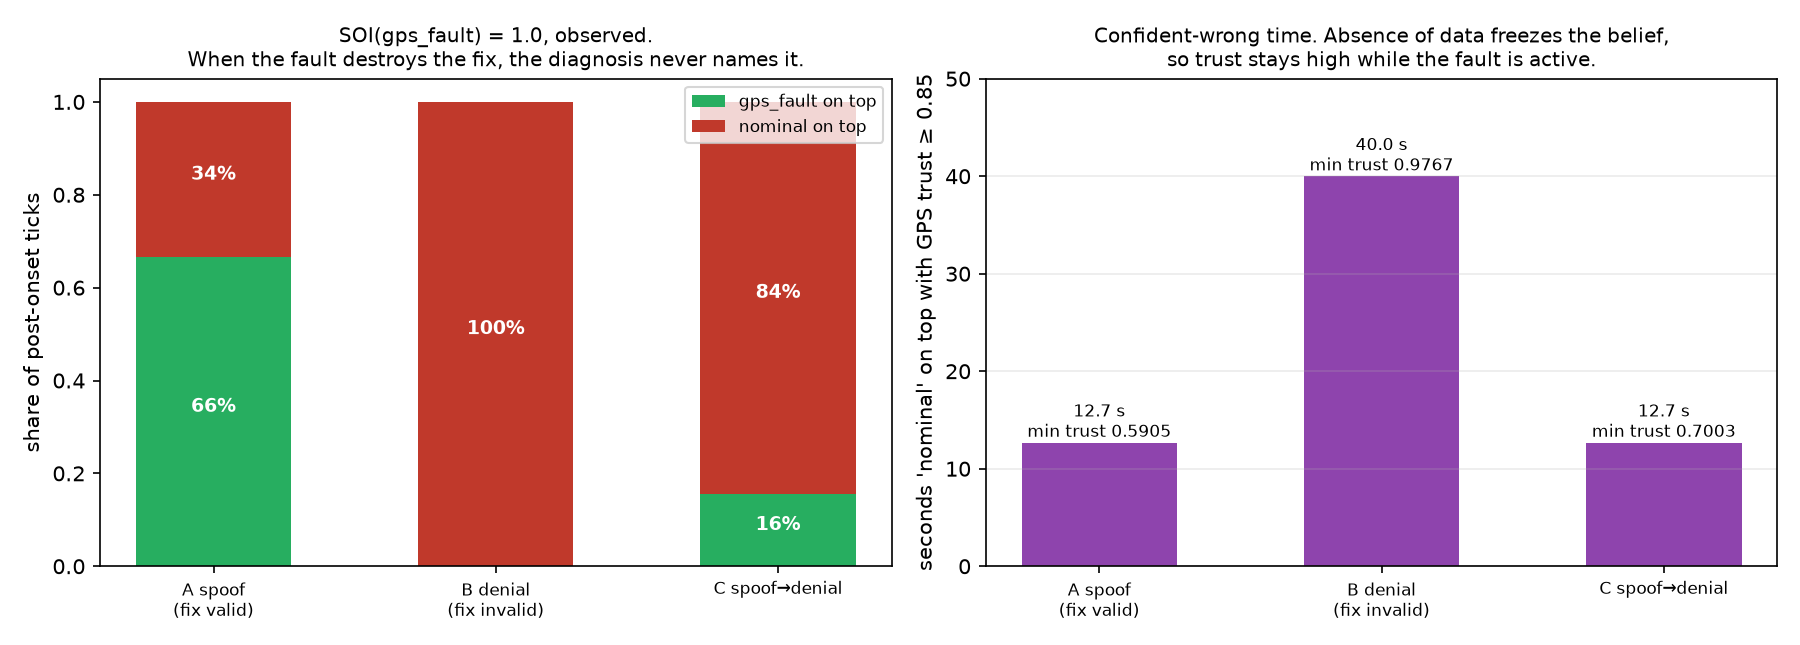
\includegraphics[width=\textwidth]{figures/wp_c4_self_occlusion.png}
\caption{Left: share of post-onset ticks by leading hypothesis. Right:
seconds spent reporting \code{nominal} with GPS trust above the actionable
threshold, with the trust minimum annotated.}
\end{figure}

%======================================================================
\section{Containment: what is established and what is not}
\label{sec:containment}

Two conditions must be kept apart. Write $E_h$ for the features hypothesis $h$
actually references in the deployed signature matrix, $U_h$ for the set of all
physically admissible relations that could bear on $h$, and $C_h$ for the set
of features controlled by gates that $h$ itself closes.

\begin{align}
E_h &\subseteq C_h && \text{present support silenced} \label{eq:eh}\\
U_h &\subseteq C_h && \text{whole universe silenced} \label{eq:uh}
\end{align}

Condition~\eqref{eq:eh} gives effective undetectability now, for the system as
built. Condition~\eqref{eq:uh} would give irreparability: no addition of
evidence could ever repair the collapse. \textbf{We establish
\eqref{eq:eh} and we do not establish \eqref{eq:uh}.} An earlier draft of this
work did not separate them.

\paragraph{\eqref{eq:eh} holds for \code{gps\_fault}, by inspection.}
$E_{\code{gps\_fault}} = \{\code{phys\_gps}\}$, read from the signature matrix
in \code{bayes.py}. \code{phys\_gps} is gated by
$\code{gvalid} \cdot \mathbb{1}[\tau > 3]$, read from \code{online.py}, so
$\code{phys\_gps} \in C_{\code{gps\_fault}}$. A one-element subset check is the
whole proof. This is what Section~\ref{sec:measurement} measures the
consequence of.

\paragraph{\eqref{eq:uh} is not established, and cannot be by these methods.}
$U_h$ is the set of relations that could in principle be built, which is not a
finite object we can enumerate without first fixing what counts as admissible.
Any argument that every admissible GNSS relation is fix-gated is at risk of
defining admissibility so that it is. We do not have a non-circular definition
of $U_h$ and we do not claim \eqref{eq:uh}.

What we can do instead is bound $U_h$ over a set that \emph{is} finite and
enumerable, which is Section~\ref{sec:fieldset}.

\subsection{A generator-dependent sensitivity study}

A natural objection is that arm B is an artifact of a sparse signature matrix:
this system averages 2.4 features per hypothesis, and \code{gps\_fault} has
exactly one. If the collapse disappears once hypotheses carry more evidence,
the finding is about sparsity and not about gating.

We tested this by synthesising signature matrices over the same gate structure
at densities from 1 to 8 features per hypothesis, 400 draws per cell, with one
designated hypothesis closing \code{gvalid}. Two arms differ only in where
that hypothesis draws its features from.

\begin{table}[h]
\centering
\small
\begin{tabular}{lrrrr}
\toprule
Features per hypothesis & \multicolumn{2}{c}{Arm A: uniform draw} &
  \multicolumn{2}{c}{Arm B: draws from gated set} \\
& mean gap & $P(\text{gap}>0)$ & mean gap & $P(\text{gap}>0)$ \\
\midrule
1 & 0.0264 & 0.185 & 0.1018 & 0.713 \\
2 & 0.0050 & 0.037 & 0.1400 & 0.980 \\
3 & 0.0011 & 0.007 & 0.1425 & 0.998 \\
4 & 0.0004 & 0.003 & 0.1425 & 0.998 \\
5 & \textbf{0.0000} & \textbf{0.000} & \textbf{0.1429} & \textbf{1.000} \\
6--8 & 0.0000 & 0.000 & \textbf{0.1429} & \textbf{1.000} \\
\bottomrule
\end{tabular}
\caption{The gap $\kappa(S_{\mathrm{eff}}) - \kappa(S)$ against signature
density. Arm A collapses to zero by density 5. Arm B saturates at $1/7$, this
system's value, at every density.}
\label{tab:density}
\end{table}

Arm A confirms the objection for a generator that draws hypothesis evidence
freely: the gap vanishes with density. Arm B does not: it saturates at
$0.1429 = 1/7$ with the designated hypothesis fully silenced in 100\% of draws
at every density.

\textbf{What this does and does not show.} It is a statement about two
generators, not about the world. Arm A shows that the feature-density argument
against arm B succeeds when the generator draws freely. Arm B shows that the
same argument fails when the generator enforces containment. Which generator
describes a real system is a separate question, and the deployed system's is
arm B's for \code{gps\_fault} by \eqref{eq:eh}. It is a sensitivity study, and
it is not evidence for \eqref{eq:uh}.

\begin{figure}[h]
\centering
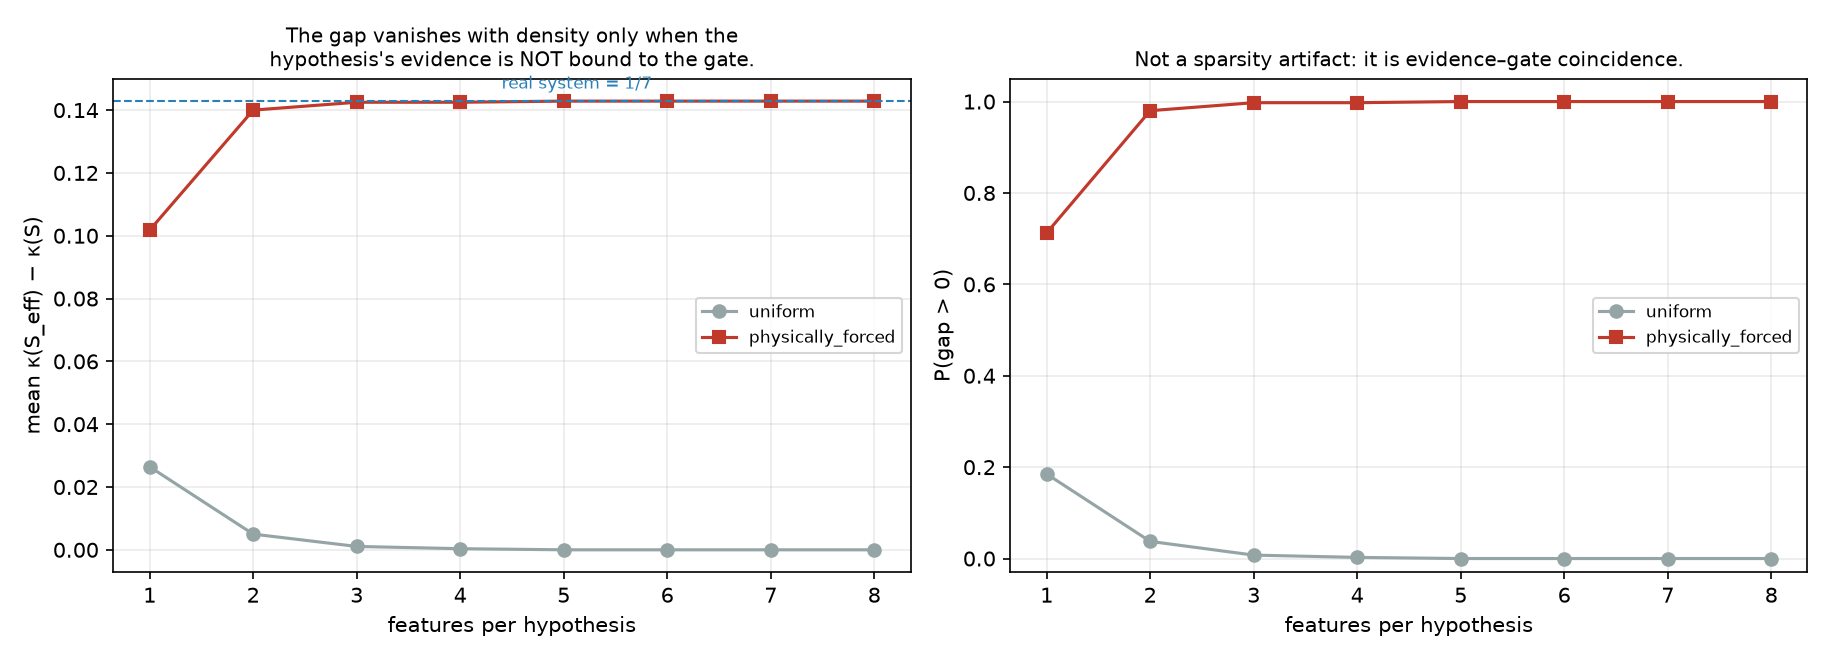
\includegraphics[width=\textwidth]{figures/wp_c4_sparsity_probe.png}
\caption{The density sweep. Left: mean gap. Right: probability the gap is
positive.}
\end{figure}

\subsection{The interior is a threshold, not a slope}
\label{sec:knifeedge}

Arms A and B are corners. We swept the interior: let a fraction $\rho$ of the
designated hypothesis's features lie inside $C_h$ and $1-\rho$ outside, at
densities 1, 2, 3, 4, 6 and 8, 400 draws per cell.

The result is a threshold at $\rho = 1$. With every feature inside $C_h$ the
hypothesis is absorbed into the nominal class in 100\% of draws; with
\emph{exactly one} feature outside, it is absorbed in 0\% of draws. The drop is
1.000 at every density tested. Effective undetectability does not degrade
gracefully with partial containment; it requires full containment of the
present support.

The engineering statement this licenses is narrower and more useful than
anything about universes: \textbf{one ungated relation suffices}. That is a
checkable design requirement, and Section~\ref{sec:repair} costs it out.

\begin{figure}[h]
\centering
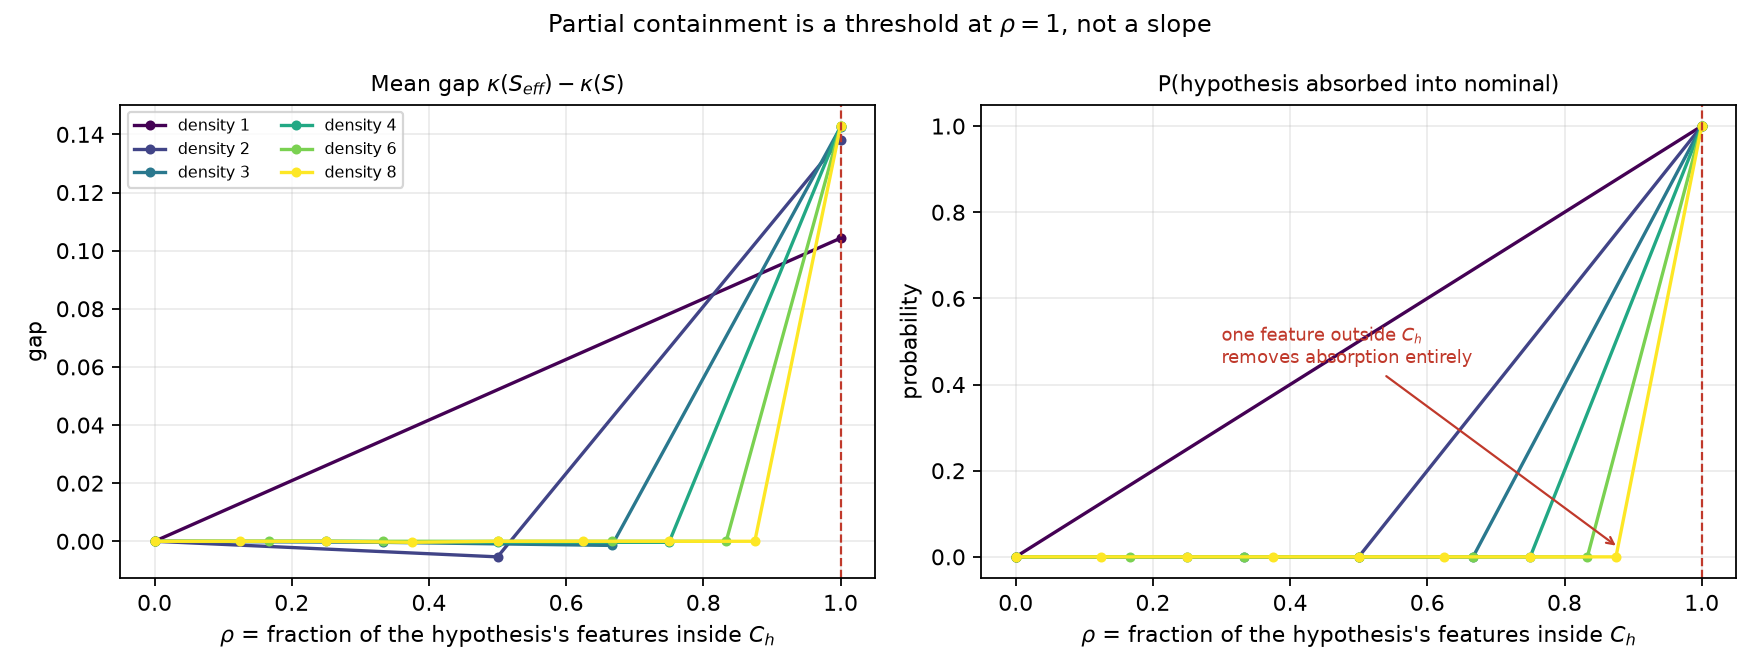
\includegraphics[width=\textwidth]{figures/wp_c6_gap_surface.png}
\caption{The interior of the containment sweep. Left: mean gap against
$\rho$. Right: probability the designated hypothesis is absorbed into the
nominal class. The transition at $\rho = 1$ is a step at every density.}
\end{figure}

\paragraph{A correction to our own reasoning.} An earlier note in this project
justified $\Pi(S_{\mathrm{eff}})$ being no finer than $\Pi(S)$ by observing
that $S_{\mathrm{eff}} \le S$ entrywise, so equal columns stay equal. That
justification is wrong in general. Entrywise domination preserves column
equality under \emph{uniform} row deletion, but per-hypothesis silencing is
\emph{column-dependent}: two hypotheses sharing a column in $S$ separate in
$S_{\mathrm{eff}}$ when only one of them silences, and the partition gets
finer. Searching 200\,000 random draws found 483 counterexamples, a rate of
0.24\%. The deployed matrix is unaffected, because \code{gps\_fault} is the
only hypothesis that silences anything and its column is unique, so no shared
column can be broken. The computational verification on the real matrix stands;
the general argument does not.

\subsection{A bound on the universe over the ingested field set}
\label{sec:fieldset}

We cannot enumerate $U_{\code{gps\_fault}}$. We can enumerate the relations
derivable from the telemetry fields the ingestion path actually reads, because
that field set is finite and closed. Reading the field list mechanically from
\code{ulog\_source.py}, six relations in the edge library span the GPS node.

\begin{table}[h]
\centering
\small
\begin{tabular}{llc}
\toprule
Relation & Spans & In $C_{\code{gps\_fault}}$ \\
\midrule
\code{altitude\_baro}           & baro, gps & yes \\
\code{velocity\_gps\_doppler\_0} & imu0, gps & yes \\
\code{velocity\_gps\_doppler\_1} & imu1, gps & yes \\
\code{heading\_course}          & mag, gps  & yes \\
\code{phys\_gps}                & gps       & yes \\
\code{temp\_gps}                & gps       & \textbf{no} \\
\bottomrule
\end{tabular}
\caption{GPS-spanning relations over the currently ingested field set. Five of
six are \code{gvalid}-gated.}
\label{tab:fieldset}
\end{table}

Formal containment over this field set is therefore \emph{false}: one relation
sits outside. But a relation outside $C_h$ is only an escape if its value
responds to the fault. Running the deployed pipeline clean and under denial on
the same truth and seed, \code{temp\_gps} consistency over the fault window is
bit-identical between the two runs (mean 0.9155, min 0.640319, max 1.0 in
both) while the GPS channel's fresh fraction falls from 1.0 to 0.001597. The
temporal predictor is computed from the channel history and never consults
channel validity, so a dropout leaves the underlying series and therefore the
residual untouched. \code{temp\_gps} is ungated and carries no information
about denial.

\textbf{The scoped statement we can defend:} over the currently ingested
telemetry field set, formal containment is incomplete by one relation and
\emph{effective} containment is complete. This is weaker than \eqref{eq:uh} and
much stronger than nothing, and it is defensible because the enumeration is
mechanical and the field set is closed.

It also names the escape route precisely. Every GPS-spanning relation
buildable from the ingested fields depends on position, velocity or altitude,
all of which are meaningless without a fix and are gvalid-gated by
construction. The fields that could support a relation surviving fix loss are
\code{satellites\_used}, \code{noise\_per\_ms}, \code{jamming\_indicator},
\code{hdop}, \code{vdop}, \code{s\_variance\_m\_s} and \code{eph}/\code{epv},
and the ingestion path reads none of them.

\begin{figure}[h]
\centering
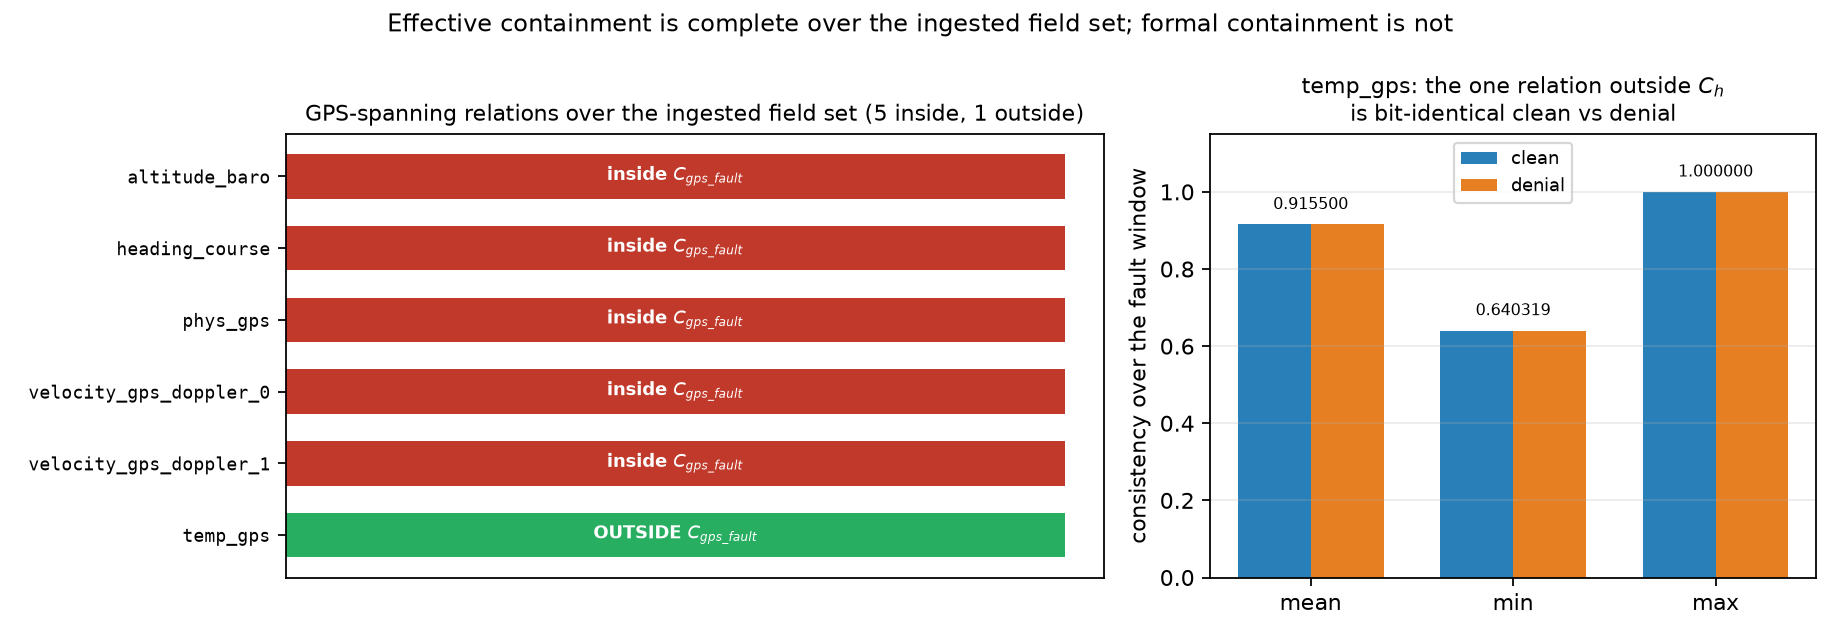
\includegraphics[width=\textwidth]{figures/wp_c6_field_set_universe.png}
\caption{Left: the six GPS-spanning relations, by whether \code{gvalid}
controls them. Right: \code{temp\_gps}, the one relation outside
$C_{\code{gps\_fault}}$, takes bit-identical values clean and under denial.}
\end{figure}

%======================================================================
\section{Gate closure frequency, measured against a real autopilot}
\label{sec:qgvalid}

Everything above is structural: it says what can happen, not how often. The
quantity that converts it into a risk statement is
$q_{\mathrm{gvalid}} \mid h = P(\code{gvalid}\ \text{closed at a tick} \mid h)$,
and it cannot be estimated from the public log corpus because that corpus is
unannotated and the conditioning variable does not exist in it.

We obtained the label by controlled injection instead. A full ArduCopter
autopilot runs in software-in-the-loop with its own EKF, its own GPS driver
and its own MAVLink stream; the deployed trust layer ingests that stream
through the production adapter, and the gate trace is the layer's own
\code{gvalid} read out of its per-tick edge record rather than recomputed. Four
arms of six flights each share the same six flight profiles, so the design is
matched. Each flight arms, climbs to 20\,m, flies a square, and receives its
injection at $t = 60$\,s; the conditioning window is $[60, 85]$\,s.
Pre-registration, stopping rules and the estimator follow a specification
fixed before the campaign ran.

\begin{table}[h]
\centering
\small
\begin{tabular}{lrrrl}
\toprule
Arm & Monitored ticks & Closed & $q_{\mathrm{gvalid}}$ & Injection reached the
receiver \\
\midrule
\code{nominal}  & 3744 & 0    & \textbf{0.000} & (no injection) \\
\code{denial}   & 3744 & 3684 & \textbf{0.984} & satellites 9.93 $\to$ 3.05 \\
\code{glitch}   & 3744 & 0    & \textbf{0.000} & position step 1.1 $\to$
62--76\,m \\
\code{degraded} & 3744 & 3672 & \textbf{0.981} & satellites 9.93 $\to$ 0.17 \\
\bottomrule
\end{tabular}
\caption{Gate closure by fault class, 6 flights per arm. The right column is
the control that distinguishes a null result from an injection the autopilot
ignored.}
\label{tab:qgvalid}
\end{table}

Three things follow, and the third is the one that changes the paper.

\paragraph{The gate never closed in healthy flight.} Zero closures in 3744
monitored ticks. By the pre-registered stopping rule a zero denominator makes
the ratio unbounded above, so we report the one-sided statement only and no
interval. This is also the weakest of the three results: the simulated receiver
does not spontaneously lose a fix, so a nominal rate of zero is a property of
the generator before it is a statement about flight.

\paragraph{Denial closes the gate, end to end, on a real autopilot.}
$q_{\mathrm{gvalid}} \mid \code{denial} = 0.984$, and the diagnosis over the
same window reports \code{nominal} at $p = 0.977$ with \code{gps\_fault} at
$p = 0.0227$, while the failsafe reaches CAUTION at $t = 61.5$\,s through the
freshness disjunct. That reproduces Section~\ref{sec:measurement} on a
different generator, with a different vehicle model, a different EKF and the
production ingestion adapter in the path. It is confirmation of the mechanism,
not evidence about frequency: \code{SIM\_GPS\_DISABLE} switches the fix flag
off, so a high closure rate under it is close to tautological.

\paragraph{A GNSS fault that keeps the fix does not close the gate.} This is
the informative arm. A position glitch of 62 to 76\,m, with ten satellites
still reported and the fix retained, produced \textbf{zero} gate closures in
3744 ticks. For that fault class the design-time and effective partitions
coincide, so the self-occlusion of Section~\ref{sec:measurement} does not
arise at all: the evidence stays available.

The layer did not use it. GPS trust fell only to 0.906--0.934 against a
\code{nav\_caution} threshold of 0.75, no failsafe transition occurred, and the
diagnosis stayed at \code{nominal} $p = 0.9997$. \textbf{That is a different
failure mode from the one this paper is about} and we do not merge them: the
first is evidence destroyed by gating, the second is evidence present and not
acted on. We report the observation and claim nothing about its cause; a
constant position offset leaves the velocity residual intact after one sample,
which is a plausible explanation we have not tested.

\paragraph{What this bounds.} Self-occlusion is specific to fix-loss faults,
not to GNSS faults in general. Both arms that removed the fix closed the gate;
the arm that kept it did not. The scope of Section~\ref{sec:measurement} is
therefore narrower than an unqualified reading would suggest, and this campaign
is what narrows it.

\begin{figure}[h]
\centering
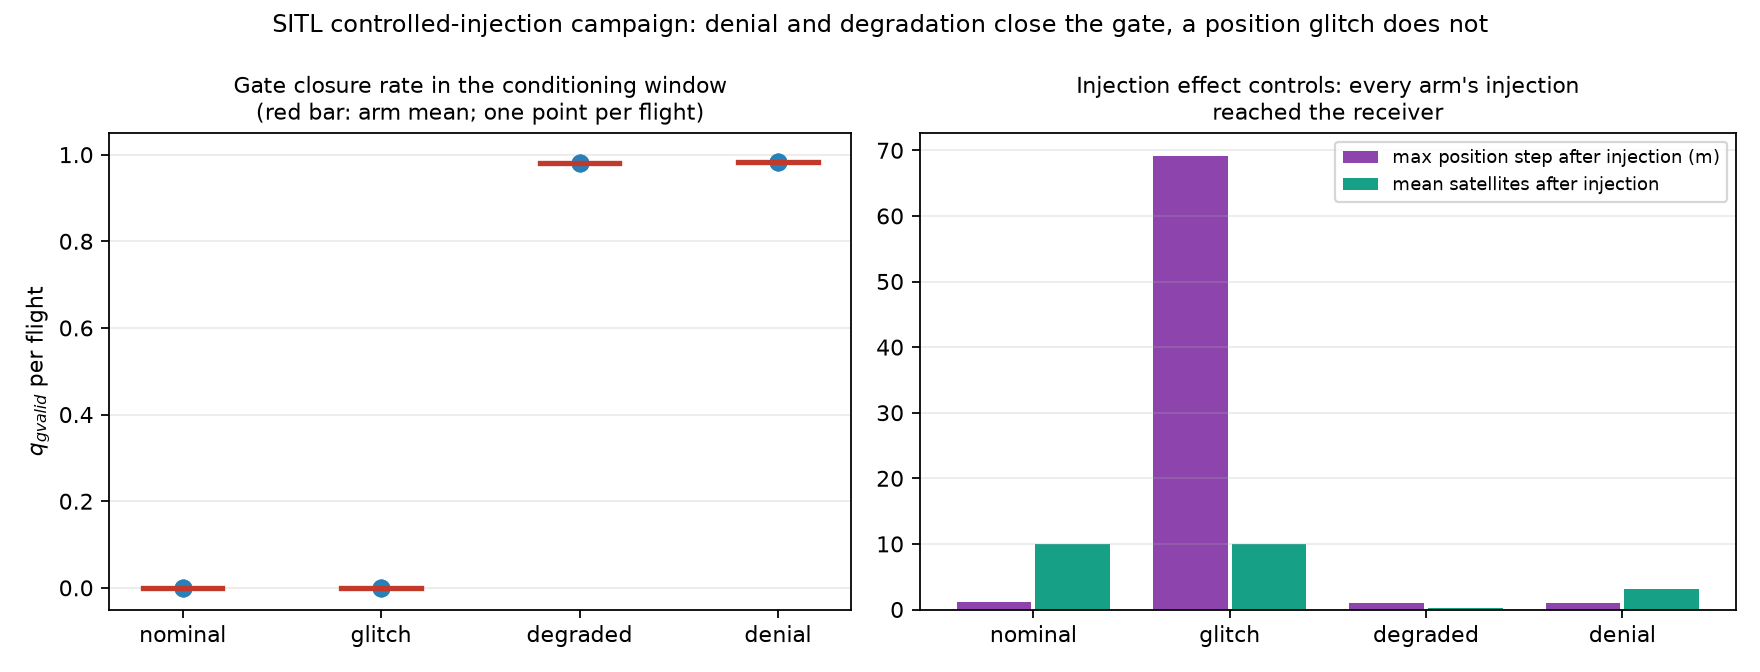
\includegraphics[width=\textwidth]{figures/wp_c6_q_gvalid_campaign.png}
\caption{Left: per-flight closure rate by arm. Right: the injection-effect
controls.}
\end{figure}

\paragraph{Limits of this campaign, stated with the result.} The flights are
near-replicates: varying home site and wind changed the trajectory but not the
gate timing, so the per-flight statistic is identical across flights in every
arm and the bootstrap interval collapses to a point. That interval is a
statement about simulator determinism and not about estimate precision, and we
report it as degenerate rather than as narrow. The receiver is simulated
throughout. \code{SIM\_GPS\_NUMSATS} $= 4$ dropped the fix in this simulator
where a real receiver may hold one. Nothing here is a measurement of real
GNSS environments.

%======================================================================
\section{Chatter resonance}
\label{sec:chatter}

Exponential smoothing with coefficient $\alpha_s$ has a characteristic time
constant $1/\alpha_s$. A gate that toggles on that timescale should maximise
label instability: faster toggling is averaged out, slower toggling lets the
accumulator settle in each state. With $\alpha_s = 0.06$ the predicted peak is
at $1/\alpha_s = 16.67$ frames.

We swept gate closure duration from 1 to 100 frames against the deployed
diagnosis kernel, holding the evidence pattern fixed so that every label
change is caused by availability alone. The observed peak is at 21 frames with
95 top-label changes per 2000 frames, against 1 to 3 changes at durations
below 18. The prediction holds on the implementation.

\begin{figure}[h]
\centering
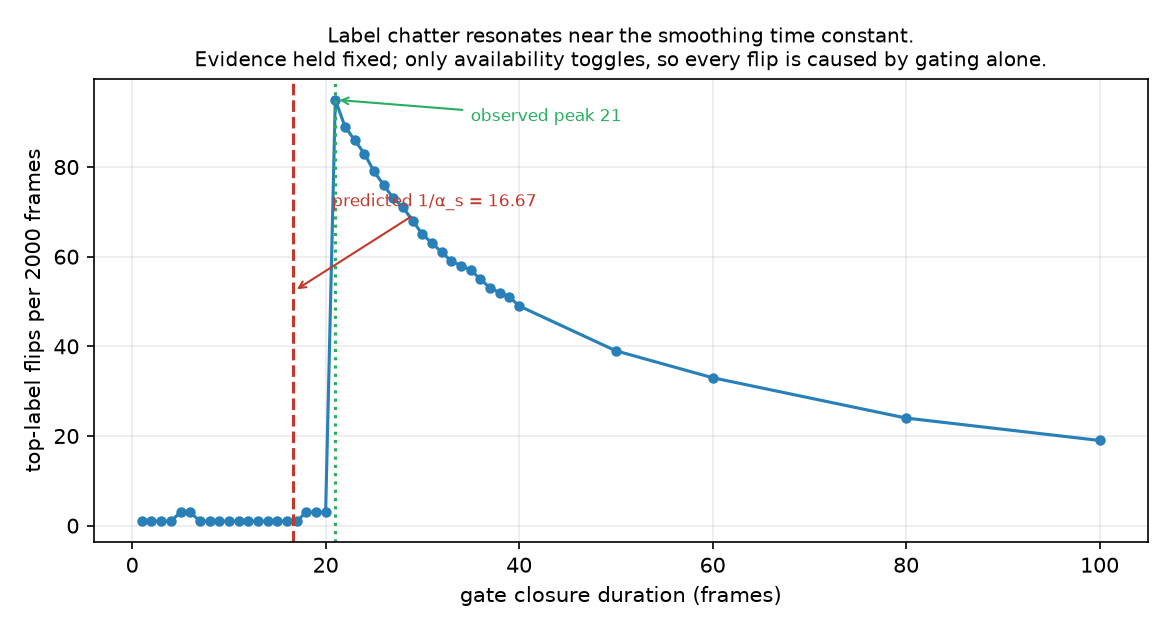
\includegraphics[width=0.85\textwidth]{figures/wp_c4_chatter_resonance.png}
\caption{Top-label changes against gate closure duration. Evidence held fixed,
so every change is caused by gating.}
\end{figure}

A methodological note. Our first attempt at this sweep made every feature
anomalous, which allowed a multi-feature hypothesis to lead whether the gate
was open or closed, and produced zero label changes at every duration. That
null result was a property of the probe, not of the system. The gated feature
must be decisive for the leading label or there is nothing to observe.

%======================================================================
\section{A design rule and its enforcement}
\label{sec:rule}

The measurement generalises into a check any gated diagnostic system can run:

\begin{quote}
A feature intended to discriminate hypothesis $h$ must not be gated by a gate
that $h$ closes.
\end{quote}

Auditing this system's 19 signature entries gives 18 clean and one violation:
\code{gps\_fault} / \code{phys\_gps} / \code{gvalid}. The violation is fatal
rather than merely weakening because \code{phys\_gps} is that hypothesis's sole
feature, so the effective signature empties rather than thins.

The rule is enforced in the project's test suite. The test pins the violation
list exactly: a new violation fails the build, and the known violation
disappearing also fails, so a silent repair cannot land without the record
being updated in the same commit. This is the transferable engineering output
of the work. It requires only a signature matrix and a gate-to-feature map,
both of which any gated diagnostic system already has.

%======================================================================
\section{A repair, measured}
\label{sec:repair}

A second collision existed: \code{imu0\_bias\_drift} and
\code{imu1\_bias\_drift} shared the signature $\{\code{redundant\_imu}\}$
whenever the motor edges gated off at disarm, because their distinguishing
features were both \code{armed\_gate}-controlled. The repair is one entry:
\code{attitude\_gravity\_mag} added to \code{imu0\_bias\_drift}. It compares
magnetometer heading against \code{imu0}-integrated yaw, so an \code{imu0}
bias corrupts it and an \code{imu1} bias does not, and it is ungated, which is
the property that matters.

Measured before and after over the full configuration lattice:

\begin{table}[h]
\centering
\small
\begin{tabular}{lrr}
\toprule
& Before & After \\
\midrule
$\kappa_{\max}$ at full instrumentation & 0.2857 & \textbf{0.1429} \\
Decision-relevant pairs exposed at full instrumentation & 2 & \textbf{1} \\
New collisions across 1232 reachable configurations & --- & \textbf{none} \\
Pairs with an order-one cut set & 7 & \textbf{6} \\
Components in any order-one cut set & 9 & \textbf{7} \\
\code{imu0}/\code{imu1} minimum cut set size & 1 & \textbf{2} \\
Peak posterior for \code{imu0\_bias\_drift} & 0.9861 & \textbf{0.9203} \\
\bottomrule
\end{tabular}
\caption{The repair. Cut-set analysis follows
\cite{hurdle2007faulttree,reeves2019sensorselection}.}
\end{table}

\textbf{The cost is real and we report it.} Peak posterior for the target
hypothesis falls by 0.066, because a larger LOW set requires more features to
be simultaneously anomalous. Detection latency and minimum trust are unchanged
on all five scripted fault scenarios, the clean scenario produces zero false
positives before and after, and the committed campaign artifact regenerates
bit-identical.

We also checked the obvious concern that routing IMU discrimination through
the magnetometer creates a new single point of diagnostic failure. It does
not: \code{mag} was already an order-one cut set for one pair before the change
and remains exactly that, while \code{armed\_gate} and \code{motor\_esc}
dropped out of the order-one set entirely.

%======================================================================
\section{Limitations}
\label{sec:limits}

\paragraph{The corpus is unannotated.} The 26 public flight logs used
elsewhere in this project carry no ground-truth health labels. No detection
performance on real flight data is claimed anywhere in this paper. The
measurements in Sections~\ref{sec:measurement} and \ref{sec:chatter} are on
simulated fault injection into the deployed pipeline.

\paragraph{Closure attribution is derived, not observed.}
$\mathrm{closes}(h,g)$ comes from reading the gate predicate in source plus the
physical fault model. If a fault closes a gate in flight that the model says it
does not, Equation~\ref{eq:seff} is wrong in the optimistic direction and the
real gap is larger than reported.

\paragraph{Structural, not statistical.} $\kappa$ bounds structural
indistinguishability. Two hypotheses in one observable class may still separate
on residual magnitude or variance. In arm B they did not, but that is one
scenario and not a proof.

\paragraph{The one frequency we measure is measured in a simulator.}
Section~\ref{sec:qgvalid} is the only frequency in this paper, and its
generator is ArduPilot SITL. No closure rate on real flight data is claimed
anywhere. The public corpus cannot supply one: it is unannotated, so the
conditioning variable does not exist in it, and reporting an unconditional
closure rate as a substitute would mix hypotheses in unknown proportion and
bound nothing. We have specified the real-telemetry measurement separately and
have not performed it.

\paragraph{The governing objection, stated in full.} The strongest objection to
Section~\ref{sec:containment} is this one, and we reproduce it as it was put to
us:

\begin{quote}
``Unless the admissible evidence universe is defined independently, shown
complete, and difficult to compute, this is a modeling observation rather than
a new theorem.''
\end{quote}

We do not defeat it. The admissible evidence universe $U_h$ is not defined
independently here, is not shown complete, and is not difficult to compute
because it is not computed at all. Every part of the objection lands.

Our answer is to concede it and narrow the claim. We assert \eqref{eq:eh},
which is a one-element subset check on committed source. We assert the scoped
enumeration of Section~\ref{sec:fieldset}, which is complete over a closed
finite field set and says so. We do not assert \eqref{eq:uh}. What survives is
a modeling observation about one deployed system plus a measurement of what it
does, and that is what this paper claims to be.

The measurement in Section~\ref{sec:measurement} does not depend on defeating
the objection. It is a recording of what a deployed system did under a fault,
and it would read the same if $U_h$ were never definable.

\paragraph{Priority is not asserted anywhere.} The general mechanism of
fault-state-dependent observation loss belongs to
\cite{dong2024statedependent}. Section~\ref{sec:containment} states a property
of one system's structure and nothing more. We assert no priority.

\paragraph{Simulation fidelity, and what the campaign did about it.} The
internal fault model produces denial by invalidating the fix flag, and real
GNSS degradation is richer. Section~\ref{sec:qgvalid} addresses this directly
by adding fault classes that keep the fix, and the result is that the gate
does not close for them. The remaining gap is that the ArduPilot receiver
model is still a model: it dropped the fix at four satellites where a real
receiver may hold one, and it reproduces neither gradual carrier-to-noise
decay nor multipath.

\paragraph{Six flights per arm are not six independent observations.} The
flight profiles differ in home site and wind but the injection is scripted and
the simulated receiver is deterministic, so the per-flight closure rate is
identical across flights within each arm. The bootstrap interval is therefore
degenerate and carries no information about precision. We report it as such.

%======================================================================
\section{Claim table}
\label{sec:claims}

\begin{longtable}{p{0.52\textwidth}p{0.40\textwidth}}
\toprule
Claim & Status \\
\midrule
\endhead
Under 40\,s GPS denial the diagnosis reports \code{nominal} throughout and
never names \code{gps\_fault} & EMPIRICAL RESULT, simulated fault injection
into the deployed pipeline \\
GPS trust reads 0.9767 over the same window & EMPIRICAL RESULT \\
The failsafe still reaches CAUTION via the freshness disjunct & EMPIRICAL
RESULT \\
$\kappa(S)=0.000$, $\kappa(S_{\mathrm{eff}})=0.143$ for this system & VERIFIED
FACT, computed from committed artifacts \\
$\Pi(S_{\mathrm{eff}})$ is no finer than $\Pi(S)$ for this system & VERIFIED
FACT by computation. The entrywise-domination \emph{argument} for it in general
is REFUTED: 483 counterexamples in 200\,000 draws \\
$E_{\code{gps\_fault}} \subseteq C_{\code{gps\_fault}}$ & VERIFIED FACT,
one-element subset check on committed source \\
$U_{\code{gps\_fault}} \subseteq C_{\code{gps\_fault}}$ (irreparability) & NOT
ESTABLISHED and not claimed. Requires a non-circular definition of the
admissible evidence universe \\
Effective containment is complete over the currently ingested field set &
VERIFIED FACT, mechanical enumeration of 6 GPS-spanning relations; formal
containment is incomplete by one \\
Effective undetectability is a threshold at $\rho=1$ & EMPIRICAL RESULT over
synthesised matrices; one feature outside $C_h$ removes absorption entirely \\
Chatter peaks near $1/\alpha_s$ & EMPIRICAL RESULT, predicted 16.67 frames,
observed 21 \\
The repair halves $\kappa_{\max}$ with no new collision & EMPIRICAL RESULT
over 1232 configurations \\
The design rule is checkable and enforced & VERIFIED FACT, in the test suite \\
Any framework in Section~\ref{sec:related} is ours & REFUTED. All are prior
work and cited as such \\
Detection performance on real flight data & NOT CLAIMED. Corpus is unannotated \\
$q_{\mathrm{gvalid}}$ is 0.984 under denial and 0.981 under constellation loss
& EMPIRICAL RESULT, ArduPilot SITL controlled injection, 6 flights per arm \\
$q_{\mathrm{gvalid}}$ is 0.000 under a 62--76\,m position glitch that keeps the
fix & EMPIRICAL RESULT. Self-occlusion is specific to fix-loss faults \\
$q_{\mathrm{gvalid}}$ is 0.000 in healthy flight & EMPIRICAL RESULT, but the
simulated receiver never loses a fix on its own, so this bounds the simulator
before it bounds flight \\
Closure frequency of \code{gvalid} on real telemetry & UNMEASURED. No real
logs are reachable and the corpus carries no labels \\
A 62--76\,m position glitch raised no failsafe transition & EMPIRICAL RESULT.
A separate failure mode from self-occlusion; cause not established \\
\bottomrule
\end{longtable}

%======================================================================
\section{Conclusion}

A deployed aerospace diagnostic layer reported healthy for 40 seconds while a
fault it was built to catch destroyed the evidence that would name it, with
its trust channel independently agreeing. The escalation path held, through a
mechanism that does not consult the diagnosis. We report the measurement, the
structural condition that makes it irreparable by adding evidence, a design
rule that catches the pattern, and a repair to a second instance with its cost.
We claim no mathematics. The frameworks were already there; what was missing
was somebody running the measurement on a real system and reporting what came
back.

\bibliographystyle{plain}
\bibliography{refs}

\end{document}
